% questions.tex —— 2012 年·全国新课标卷·理科 · 题目内容片段（无答案）
% 由 tools/generate_projects.py 依来源总账自 2012/2012_数学真题_全国新课标理_试题.md 生成，勿手改（改源 MD 后重跑）


\gkpart{数学}

\begin{gknotice}
\textbf{来源说明}：本题面依据固定源 PDF 的两页 A3 题面逐题转录。PDF 第 1 页对应原卷印刷页 755，含选择题 1–12、填空题 13–16 和解答题 17；PDF 第 2 页对应原卷印刷页 756，含解答题 18–24。

\textbf{解析归属}：固定源不附答案或解析；配套答案与解析均由本库按本题面独立复算。

\textbf{图形说明}：第 6、10、15、19、22 题的流程图、函数图象选项、电路图、三棱柱图和圆内几何图由项目内 TikZ 矢量源重绘。下列 Markdown 使用逻辑 PNG 标记供后续生成器映射，仓库不保存 PNG/JPEG/SVG 图像。
\end{gknotice}

\gkpart{一、选择题}

\begin{question}
\gkti{1}已知集合 $A=\{1,2,3,4,5\}$，$B=\{(x,y)\mid x\in A,\ y\in A,\ x-y\in A\}$，则 $B$ 中所含元素的个数为\mbox{（　　）}

\begin{gkopts}(4)
\task （A）$3$
\task （B）$6$
\task （C）$8$
\task （D）$10$
\end{gkopts}

\end{question}
\begin{question}
\gkti{2}将 $2$ 名教师、$4$ 名学生分成 $2$ 个小组，分别安排到甲、乙两地参加社会实践活动，每个小组由 $1$ 名教师和 $2$ 名学生组成，不同的安排方案共有\mbox{（　　）}

\begin{gkopts}(4)
\task （A）$12$ 种
\task （B）$10$ 种
\task （C）$9$ 种
\task （D）$8$ 种
\end{gkopts}

\end{question}
\begin{question}
\gkti{3}下面是关于复数 $z=\dfrac{2}{-1+i}$ 的四个命题：

$p_1$：$|z|=2$；$p_2$：$z^2=2i$；$p_3$：$z$ 的共轭复数为 $1+i$；$p_4$：$z$ 的虚部为 $-1$。其中的真命题为\mbox{（　　）}

\begin{gkopts}(4)
\task （A）$p_2,p_3$
\task （B）$p_1,p_2$
\task （C）$p_2,p_4$
\task （D）$p_3,p_4$
\end{gkopts}

\end{question}
\begin{question}
\gkti{4}设 $F_1,F_2$ 是椭圆 $E:\dfrac{x^2}{a^2}+\dfrac{y^2}{b^2}=1$（$a>b>0$）的左、右焦点，$P$ 为直线 $x=\dfrac{3a}{2}$ 上一点，$\triangle F_2PF_1$ 是底角为 $30^\circ$ 的等腰三角形，则 $E$ 的离心率为\mbox{（　　）}

\begin{gkopts}(4)
\task （A）$\dfrac12$
\task （B）$\dfrac23$
\task （C）$\dfrac34$
\task （D）$\dfrac45$
\end{gkopts}

\end{question}
\begin{question}
\gkti{5}已知 $\{a_n\}$ 为等比数列，$a_4+a_7=2$，$a_5a_6=-8$，则 $a_1+a_{10}=$\mbox{（　　）}

\begin{gkopts}(4)
\task （A）$7$
\task （B）$5$
\task （C）$-5$
\task （D）$-7$
\end{gkopts}

\Needspace{0.4\textheight}
\end{question}
\begin{question}
\gkti{6}如果执行下面的程序框图，输入正整数 $N$（$N\geqslant2$）和实数 $a_1,a_2,\cdots,a_N$，输出 $A,B$，则\mbox{（　　）}
\nopagebreak[4]
\begin{center}\begin{tikzpicture}[
  >=stealth,
  node distance=7mm and 12mm,
  every node/.style={font=\small},
  scale=.78,
  transform shape
]
\node[draw,rounded corners,minimum width=18mm,minimum height=7mm] (start) {开始};
\node[draw,trapezium,trapezium left angle=75,trapezium right angle=105,
      minimum width=43mm,minimum height=7mm,below=of start]
      (input) {输入 $N,a_1,a_2,\ldots,a_N$};
\node[draw,minimum width=38mm,minimum height=7mm,below=of input]
      (init) {$k=1,\ A=a_1,\ B=a_1$};
\node[draw,minimum width=20mm,minimum height=7mm,below=of init]
      (read) {$x=a_k$};
\node[draw,diamond,aspect=2.2,below=of read,minimum width=25mm,minimum height=8mm]
      (max) {$x>A$};
\node[draw,minimum width=18mm,minimum height=7mm,right=of max]
      (setmax) {$A=x$};
\node[draw,diamond,aspect=2.2,below=of max,minimum width=25mm,minimum height=8mm]
      (min) {$x<B$};
\node[draw,minimum width=18mm,minimum height=7mm,left=of min]
      (setmin) {$B=x$};
\node[draw,diamond,aspect=2.2,below=of min,minimum width=25mm,minimum height=8mm]
      (done) {$k\geqslant N$};
\node[draw,minimum width=25mm,minimum height=7mm,right=of done]
      (inc) {$k=k+1$};
\node[draw,trapezium,trapezium left angle=75,trapezium right angle=105,
      minimum width=25mm,minimum height=7mm,below=of done]
      (out) {输出 $A,B$};
\node[draw,rounded corners,minimum width=18mm,minimum height=7mm,below=of out]
      (end) {结束};

\draw[->] (start)--(input)--(init)--(read)--(max);
\draw[->] (max)--node[above]{是}(setmax)--++(0,-.65) |- (done);
\draw[->] (max)--node[right]{否}(min);
\draw[->] (min)--node[above]{是}(setmin)--++(0,-.65) |- (done);
\draw[->] (min)--node[right]{否}(done);
\draw[->] (done)--node[above]{否}(inc) |- (read);
\draw[->] (done)--node[right]{是}(out)--(end);
\end{tikzpicture}
\end{center}
\nopagebreak[4]
（A）$A+B$ 为 $a_1,a_2,\cdots,a_N$ 的和

（B）$\dfrac{A+B}{2}$ 为 $a_1,a_2,\cdots,a_N$ 的算术平均数

（C）$A$ 和 $B$ 分别是 $a_1,a_2,\cdots,a_N$ 中最大的数和最小的数

（D）$A$ 和 $B$ 分别是 $a_1,a_2,\cdots,a_N$ 中最小的数和最大的数

\Needspace{0.4\textheight}
\end{question}
\begin{question}
\gkti{7}如图，网格上小正方形的边长为 $1$，粗线画出的是某几何体的三视图，则此几何体的体积为\mbox{（　　）}
\nopagebreak[4]
\begin{center}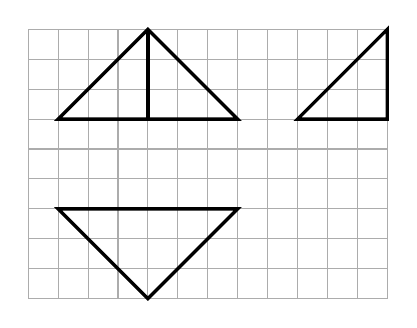
\begin{tikzpicture}[scale=.38]
  \draw[gray!65] (0,0) grid (12,9);
  \draw[very thick] (1,6)--(7,6)--(4,9)--cycle;
  \draw[very thick] (4,6)--(4,9);
  \draw[very thick] (9,6)--(12,6)--(12,9)--cycle;
  \draw[very thick] (1,3)--(7,3)--(4,0)--cycle;
\end{tikzpicture}
\end{center}
\nopagebreak[4]
\begin{gktip}
\textbf{第 7 题图形转录}：固定源印刷页 755 的网格图含三个粗线视图：左上为底边长 $6$、高 $3$ 且标出中线的等腰三角形；右上为两直角边长均为 $3$ 的直角三角形；左下为底边长 $6$、高 $3$ 的倒置等腰三角形。
\end{gktip}

\begin{gkopts}(4)
\task （A）$6$
\task （B）$9$
\task （C）$12$
\task （D）$18$
\end{gkopts}

\end{question}
\begin{question}
\gkti{8}等轴双曲线 $C$ 的中心在原点，焦点在 $x$ 轴上，$C$ 与抛物线 $y^2=16x$ 的准线交于 $A,B$ 两点，$|AB|=4\sqrt3$，则 $C$ 的实轴长为\mbox{（　　）}

\begin{gkopts}(4)
\task （A）$\sqrt2$
\task （B）$2\sqrt2$
\task （C）$4$
\task （D）$8$
\end{gkopts}

\end{question}
\begin{question}
\gkti{9}已知 $\omega>0$，函数 $f(x)=\sin\left(\omega x+\dfrac{\pi}{4}\right)$ 在 $\left(\dfrac{\pi}{2},\pi\right)$ 单调递减，则 $\omega$ 的取值范围是\mbox{（　　）}

\begin{gkopts}(2)
\task （A）$\left[\dfrac12,\dfrac54\right]$
\task （B）$\left[\dfrac12,\dfrac34\right]$
\task （C）$\left(0,\dfrac12\right]$
\task （D）$(0,2]$
\end{gkopts}

\Needspace{0.4\textheight}
\end{question}
\begin{question}
\gkti{10}已知函数 $f(x)=\dfrac{1}{\ln(x+1)-x}$，则 $y=f(x)$ 的图象大致为\mbox{（　　）}
\nopagebreak[4]
\begin{center}\begin{tikzpicture}[font=\small, x=1.05cm, y=.62cm]
  \begin{scope}
    \draw[->] (-1.25,0)--(2.65,0) node[right] {$x$};
    \draw[->] (0,-4)--(0,3.9) node[above] {$y$};
    \draw (1,-.08)--(1,.08) node[below right,inner sep=1pt] {$1$};
    \draw (-.08,1)--(.08,1) node[left,inner sep=1pt] {$1$};
    \node[below left,inner sep=1pt] at (0,0) {$O$};
    \draw[thick] (.12,3.7) .. controls (.18,2.0) and (.45,.65) .. (2.35,.15);
    \node[below] at (.65,-4.55) {(A)};
  \end{scope}
  \begin{scope}[xshift=5.1cm]
    \draw[->] (-1.25,0)--(2.65,0) node[right] {$x$};
    \draw[->] (0,-4)--(0,3.9) node[above] {$y$};
    \draw (1,-.08)--(1,.08) node[below right,inner sep=1pt] {$1$};
    \draw (-.08,1)--(.08,1) node[left,inner sep=1pt] {$1$};
    \node[below left,inner sep=1pt] at (0,0) {$O$};
    \draw[thick] (-1.05,-.10) .. controls (-.55,-.18) and (-.13,-1.2) .. (-.06,-3.8);
    \draw[thick] (.06,-3.8) .. controls (.13,-1.2) and (.55,-.18) .. (2.35,-.10);
    \node[below] at (.65,-4.55) {(B)};
  \end{scope}
  \begin{scope}[yshift=-5.25cm]
    \draw[->] (-1.25,0)--(2.65,0) node[right] {$x$};
    \draw[->] (0,-4)--(0,3.9) node[above] {$y$};
    \draw (1,-.08)--(1,.08) node[below right,inner sep=1pt] {$1$};
    \draw (-.08,1)--(.08,1) node[left,inner sep=1pt] {$1$};
    \node[below left,inner sep=1pt] at (0,0) {$O$};
    \draw[thick] (-1.05,.10) .. controls (-.55,.18) and (-.13,1.2) .. (-.06,3.8);
    \draw[thick] (.06,-3.8) .. controls (.13,-1.2) and (.55,-.18) .. (2.35,-.10);
    \node[below] at (.65,-4.55) {(C)};
  \end{scope}
  \begin{scope}[xshift=5.1cm,yshift=-5.25cm]
    \draw[->] (-1.25,0)--(2.65,0) node[right] {$x$};
    \draw[->] (0,-4)--(0,3.9) node[above] {$y$};
    \draw (1,-.08)--(1,.08) node[below right,inner sep=1pt] {$1$};
    \draw (-.08,1)--(.08,1) node[left,inner sep=1pt] {$1$};
    \node[below left,inner sep=1pt] at (0,0) {$O$};
    \draw[thick] (.06,-3.8) .. controls (.13,-1.2) and (.55,-.18) .. (2.35,-.10);
    \node[below] at (.65,-4.55) {(D)};
  \end{scope}
\end{tikzpicture}
\end{center}
\nopagebreak[4]
\begin{gkopts}(4)
\task （A）图 A
\task （B）图 B
\task （C）图 C
\task （D）图 D
\end{gkopts}

\end{question}
\begin{question}
\gkti{11}已知三棱锥 $S-ABC$ 的所有顶点都在球 $O$ 的球面上，$\triangle ABC$ 是边长为 $1$ 的正三角形，$SC$ 为球 $O$ 的直径，且 $SC=2$，则此棱锥的体积为\mbox{（　　）}

\begin{gkopts}(2)
\task （A）$\dfrac{\sqrt2}{6}$
\task （B）$\dfrac{\sqrt3}{6}$
\task （C）$\dfrac{\sqrt2}{3}$
\task （D）$\dfrac{\sqrt2}{2}$
\end{gkopts}

\end{question}
\begin{question}
\gkti{12}设点 $P$ 在曲线 $y=\dfrac12\mathrm e^x$ 上，点 $Q$ 在曲线 $y=\ln(2x)$ 上，则 $|PQ|$ 的最小值为\mbox{（　　）}

\begin{gkopts}(2)
\task （A）$1-\ln2$
\task （B）$\sqrt2(1-\ln2)$
\task （C）$1+\ln2$
\task （D）$\sqrt2(1+\ln2)$
\end{gkopts}

\end{question}
\gkpart{二、填空题}

\begin{question}
\gkti{13}已知向量 $\boldsymbol a,\boldsymbol b$ 夹角为 $45^\circ$，且 $|\boldsymbol a|=1$，$|2\boldsymbol a-\boldsymbol b|=\sqrt{10}$，则 $|\boldsymbol b|=$\gkblank{}。

\end{question}
\begin{question}
\gkti{14}设 $x,y$ 满足约束条件

\nopagebreak[4]
\[
\begin{cases}
x-y\geqslant-1,\\
x+y\leqslant3,\\
x\geqslant0,\\
y\geqslant0,
\end{cases}
\]

则 $z=x-2y$ 的取值范围为\gkblank{}。

\Needspace{0.4\textheight}
\end{question}
\begin{question}
\gkti{15}某一部件由三个电子元件按下图方式连接而成，元件 $1$ 或元件 $2$ 正常工作，且元件 $3$ 正常工作，则部件正常工作。设三个电子元件的使用寿命（单位：小时）均服从正态分布 $N(1000,50^2)$，且各个元件能否正常工作相互独立，那么该部件的使用寿命超过 $1000$ 小时的概率为\gkblank{}。
\nopagebreak[4]
\begin{center}\begin{tikzpicture}[font=\small]
  \draw (-.6,0) -- (.55,0);
  \draw (.55,0) -- (.55,1.05) -- (1.15,1.05);
  \draw (.55,0) -- (.55,-1.05) -- (1.15,-1.05);
  \draw (2.65,1.05) -- (3.25,1.05) -- (3.25,0) -- (3.85,0);
  \draw (2.65,-1.05) -- (3.25,-1.05) -- (3.25,0);
  \node[draw,minimum width=1.5cm,minimum height=.62cm] at (1.9,1.05) {元件 1};
  \node[draw,minimum width=1.5cm,minimum height=.62cm] at (1.9,-1.05) {元件 2};
  \node[draw,minimum width=1.5cm,minimum height=.62cm] at (4.6,0) {元件 3};
\end{tikzpicture}
\end{center}
\nopagebreak[4]
\end{question}
\begin{question}
\gkti{16}数列 $\{a_n\}$ 满足 $a_{n+1}+(-1)^n a_n=2n-1$，则 $\{a_n\}$ 的前 $60$ 项和为\gkblank{}。

\end{question}
\gkpart{三、解答题}

\begin{question}
\gkti{17}已知 $a,b,c$ 分别为 $\triangle ABC$ 三个内角 $A,B,C$ 的对边，$a\cos C+\sqrt3a\sin C-b-c=0$。

（1） 求 $A$；

（2） 若 $a=2$，$\triangle ABC$ 的面积为 $\sqrt3$，求 $b,c$。

\end{question}
\begin{question}
\gkti{18}某花店每天以每枝 $5$ 元的价格从农场购进若干枝玫瑰花，然后以每枝 $10$ 元的价格出售，如果当天卖不完，剩下的玫瑰花作垃圾处理。

（1） 若花店一天购进 $16$ 枝玫瑰花，求当天的利润 $y$（单位：元）关于当天需求量 $n$（单位：枝，$n\in\mathbb N$）的函数解析式；

（2） 花店记录了 $100$ 天玫瑰花的日需求量（单位：枝），整理得下表：

\begin{center}
\begingroup\setlength{\tabcolsep}{4pt}
\begin{tabular}{lrrrrrrr}
\toprule
日需求量 $n$ & 14 & 15 & 16 & 17 & 18 & 19 & 20 \\
\midrule
频数 & 10 & 20 & 16 & 16 & 15 & 13 & 10 \\
\bottomrule
\end{tabular}
\endgroup
\end{center}

以 $100$ 天记录的各需求量的频率作为各需求量发生的概率。

① 若花店一天购进 $16$ 枝玫瑰花，$X$ 表示当天的利润（单位：元），求 $X$ 的分布列、数学期望及方差；

② 若花店计划一天购进 $16$ 枝或 $17$ 枝玫瑰花，你认为应购进 $16$ 枝还是 $17$ 枝？请说明理由。

\Needspace{0.4\textheight}
\end{question}
\begin{question}
\gkti{19}如图，直三棱柱 $ABC-A_1B_1C_1$ 中，$AC=BC=\dfrac12AA_1$，$D$ 是棱 $AA_1$ 的中点，$DC_1\perp BD$。
\nopagebreak[4]
\begin{center}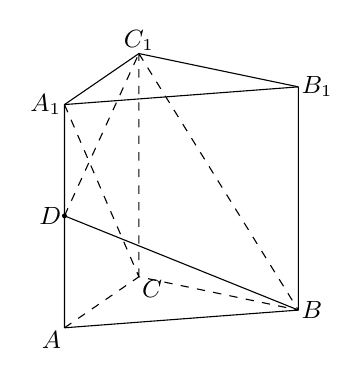
\begin{tikzpicture}[scale=.9, font=\small]
  \coordinate (A)  at (0,0);
  \coordinate (B)  at (3.3,.25);
  \coordinate (C)  at (1.05,.72);
  \coordinate (A1) at (0,3.15);
  \coordinate (B1) at (3.3,3.40);
  \coordinate (C1) at (1.05,3.87);
  \coordinate (D)  at (0,1.58);

  \draw (A)--(B) (A)--(A1) (A1)--(B1) (B)--(B1);
  \draw (A1)--(C1)--(B1);
  \draw (D)--(B);
  \draw[dashed] (A)--(C)--(B) (C)--(C1) (A1)--(C) (C1)--(B);
  \draw[dashed] (D)--(C1);
  \fill (D) circle (1pt);
  \node[below left,inner sep=1pt] at (A) {$A$};
  \node[right,inner sep=1pt] at (B) {$B$};
  \node[below right,inner sep=1pt] at (C) {$C$};
  \node[left,inner sep=1pt] at (A1) {$A_1$};
  \node[right,inner sep=1pt] at (B1) {$B_1$};
  \node[above,inner sep=1pt] at (C1) {$C_1$};
  \node[left,inner sep=1pt] at (D) {$D$};
\end{tikzpicture}
\end{center}
\nopagebreak[4]
（1） 证明：$DC_1\perp BC$；

（2） 求二面角 $A_1-BD-C_1$ 的大小。

\end{question}
\begin{question}
\gkti{20}设抛物线 $C:x^2=2py$（$p>0$）的焦点为 $F$，准线为 $l$，$A$ 为 $C$ 上一点，已知以 $F$ 为圆心、$FA$ 为半径的圆 $F$ 交 $l$ 于 $B,D$ 两点。

（1） 若 $\angle BFD=90^\circ$，$\triangle ABD$ 的面积为 $4\sqrt2$，求 $p$ 的值及圆 $F$ 的方程；

（2） 若 $A,B,F$ 三点在同一直线 $m$ 上，直线 $n$ 与 $m$ 平行，且 $n$ 与 $C$ 只有一个公共点，求坐标原点到 $m,n$ 距离的比值。

\end{question}
\begin{question}
\gkti{21}已知函数 $f(x)$ 满足

\nopagebreak[4]
\[
f(x)=f'(1)\mathrm e^{x-1}-f(0)x+\frac12x^2.
\]

（1） 求 $f(x)$ 的解析式及单调区间；

（2） 若 $f(x)\geqslant\dfrac12x^2+ax+b$，求 $(a+1)b$ 的最大值。

\Needspace{0.4\textheight}
\end{question}
\begin{question}
\gkti{22}如图，$D,E$ 分别为 $\triangle ABC$ 边 $AB,AC$ 的中点，直线 $DE$ 交 $\triangle ABC$ 的外接圆于 $F,G$ 两点。若 $CF\parallel AB$，证明：
\nopagebreak[4]
\begin{center}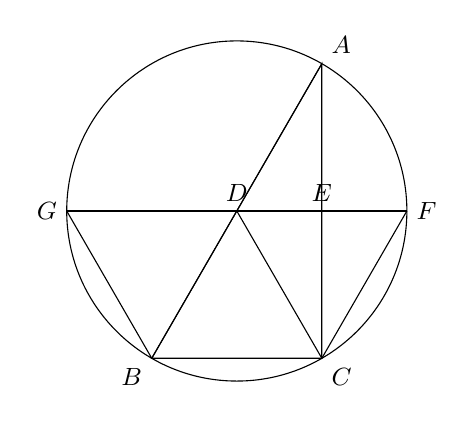
\begin{tikzpicture}[scale=.72, every node/.style={font=\small}]
  \coordinate (G) at (-3,0);
  \coordinate (F) at (3,0);
  \coordinate (A) at (1.5,2.598);
  \coordinate (B) at (-1.5,-2.598);
  \coordinate (C) at (1.5,-2.598);
  \coordinate (D) at (0,0);
  \coordinate (E) at (1.5,0);
  \draw (0,0) circle (3);
  \draw (G)--(F);
  \draw (A)--(B)--(C)--cycle;
  \draw (D)--(C);
  \draw (G)--(B);
  \draw (C)--(F);
  \draw (A)--(C);
  \draw (A)--(B);
  \node[above right] at (A) {$A$};
  \node[below left] at (B) {$B$};
  \node[below right] at (C) {$C$};
  \node[above] at (D) {$D$};
  \node[above] at (E) {$E$};
  \node[left] at (G) {$G$};
  \node[right] at (F) {$F$};
\end{tikzpicture}
\end{center}
\nopagebreak[4]
（1） $CD=BC$；

（2） $\triangle BCD\sim\triangle GBD$。

\end{question}
\begin{question}
\gkti{23}已知曲线 $C_1$ 的参数方程是

\nopagebreak[4]
\[
\begin{cases}
x=2\cos\varphi,\\
y=3\sin\varphi,
\end{cases}
\qquad(\varphi\text{ \text{是参数}}).
\]

以坐标原点为极点，$x$ 轴的非负半轴为极轴建立极坐标系，曲线 $C_2$ 的极坐标方程是 $\rho=2$，正方形 $ABCD$ 的顶点都在 $C_2$ 上，且 $A,B,C,D$ 依逆时针次序排列，点 $A$ 的极坐标为 $\left(2,\dfrac{\pi}{3}\right)$。

（1） 求点 $A,B,C,D$ 的直角坐标；

（2） 设 $P$ 为 $C_1$ 上任意一点，求 $|PA|^2+|PB|^2+|PC|^2+|PD|^2$ 的取值范围。

\end{question}
\begin{question}
\gkti{24}已知函数 $f(x)=|x+a|+|x-2|$。

（1） 当 $a=-3$ 时，求不等式 $f(x)\geqslant3$ 的解集；

（2） 若 $f(x)\leqslant|x-4|$ 的解集包含 $[1,2]$，求 $a$ 的取值范围。

\end{question}